\documentclass[onecolumn, draftclsnofoot,10pt, compsoc]{IEEEtran}
\usepackage{graphicx}
\usepackage{url}
\usepackage{setspace}
\usepackage{indentfirst}


\usepackage{geometry}
\geometry{textheight=9.5in, textwidth=7in}

% 1. Fill in these details
\def \CapstoneTeamName{		    The Apolloers}
\def \CapstoneTeamNumber{		49}
\def \GroupMemberOne{			Jonathan Ropp}
\def \GroupMemberTwo{			Shannon Sandy}
\def \GroupMemberThree{			Dean Akin}
\def \CapstoneProjectName{		Apollo 11 3D Animation}
\def \CapstoneSponsorCompany{	OMSI}
\def \CapstoneSponsorPersona{	Jim Todd}

% 2. Uncomment the appropriate line below so that the document type works
\def \DocType{		
                %Problem Statement
				Requirements Document
				%Technology Review
				%Design Document
				%Progress Report
				}
			
\newcommand{\NameSigPair}[1]{\par
\makebox[2.75in][r]{#1} \hfil 	\makebox[3.25in]{\makebox[2.25in]{\hrulefill} \hfill		\makebox[.75in]{\hrulefill}}
\par\vspace{-12pt} \textit{\tiny\noindent
\makebox[2.75in]{} \hfil		\makebox[3.25in]{\makebox[2.25in][r]{Signature} \hfill	\makebox[.75in][r]{Date}}}}
% 3. If the document is not to be signed, uncomment the RENEWcommand below
%\renewcommand{\NameSigPair}[1]{#1}

%%%%%%%%%%%%%%%%%%%%%%%%%%%%%%%%%%%%%%%
\begin{document}
\begin{titlepage}
    \pagenumbering{gobble}
    \begin{singlespace}
        \hfill 
        % 4. If you have a logo, use this includegraphics command to put it on the coversheet.
        \includegraphics[height=2cm]{OSU_horizontal_2C_O_over_B.eps}   
        \par\vspace{.2in}
        \centering
        \scshape{
            \huge CS Capstone \DocType \par
            {\large\today}\par
            \vspace{.5in}
            \textbf{\Huge\CapstoneProjectName}\par
            \vfill
            {\large Prepared for}\par
            \Huge \CapstoneSponsorCompany\par
            \vspace{5pt}
            {\Large\NameSigPair{\CapstoneSponsorPersona}\par}
            {\large Prepared by }\par
            Group\CapstoneTeamNumber\par
            % 5. comment out the line below this one if you do not wish to name your team
            \CapstoneTeamName\par 
            \vspace{5pt}
            {\Large
                \NameSigPair{\GroupMemberOne}\par
                \NameSigPair{\GroupMemberTwo}\par
                \NameSigPair{\GroupMemberThree}\par
            }
            \vspace{20pt}
        }
        \begin{abstract}
        % 6. Fill in your abstract    
        	Our group, The Apolloers, is working with Mike Bailey to create a 3D animation about the Apollo 11 Moon Landing. This animation will be put on display in OMSI during the Summer of 2019 for the 50th anniversary of the Apollo 11 mission. The project will allow viewers to see what it is like on the Moon through animated views placed throughout the scene. This document breaks the project into requirements that we will use to guide our project through the development process. 
        \end{abstract}     
    \end{singlespace}
\end{titlepage}
\newpage
\pagenumbering{arabic}
\tableofcontents
\subsection*{Revisions}
\begin{tabular} {|p{3.25cm}|p{5cm}|p{7cm}|}
\hline
Section & Original & New \\ \hline
1.2 - Scope & \begin{itemize}
  \item Animate entire mission
  \item 25 minutes
\end{itemize} & \begin{itemize}
  \item Focus on the Lunar Surface
  \item 10 minutes, allowing for questions
\end{itemize}\\ \hline
2.2 3.2 - Functions & \begin{itemize}
  \item Go through mission from launch to splashdown
\end{itemize} & \begin{itemize}
  \item Beginning and end with historic video, middle for interactive views
\end{itemize}\\ \hline
3.1 - External Interfaces & \begin{itemize}
  \item Unsure how to implement the animation at OMSI
\end{itemize} & \begin{itemize}
  \item The planetarium uses a unique script that we will translate our project into
\end{itemize}\\ \hline

\end{tabular}


% 7. uncomment this (if applicable). Consider adding a page break.
%\listoffigures
%\listoftables
\clearpage

% 8. now you write!
\section{Introduction}
Our group will be recreating the Apollo 11 mission using 3D graphics. This project is for the Oregon Museum of Science and Industry to display in their planetarium for the 50th anniversary of the Apollo 11 mission. This document contains the requirements for this project that our group and client, Jim Todd, have agreed upon. These requirements act as a definitive list of features that our project will need to implement in order for it to be considered complete. 
    \subsection{Purpose}
    The purpose of this project is to educate the general public about the Apollo 11 mission as well as to commemorate the mission's 50th anniversary. Our goal is to create the video so that the audience at OMSI will appreciate the complexity of the mission while also being entertained. 
    \subsection{Scope}
    This project will be an animation whose target audience are the people attending the planetarium at OMSI. This includes school children on a field trip, people interested in space travel, and people who are attending the planetarium to be entertained. Since the planetarium at OMSI has a large audience of diverse people, the Apollo 11 recreation will need to be accessible, entertaining, as well as realistic in order to educate the audience without boring them.
    \subsection{Overview}
    For the animation of the Apollo 11 to be considered complete the following features will need to be implemented: textured 3D objects, a variety of camera positions for the viewer, the flight path of Apollo 11, and historic audio and video to provide context. This is a general overview of the requirements for this project. The System Requirements section will go into more detail explaining  
    \subsection{Definitions}
\begin{tabular} {|l|p{13.5cm}|}
    \hline
    Term & definition \\ \hline
    API & An Application Programming Interface is a set of protocols and tools that are used to build a software application. Essentially the `building blocks' that a programmer uses to build an application.  \\ \hline
    Apollo 11 Mission & A spaceflight operated by NASA to land the first humans on the Moon, launched July 16th, 1969.  \\ \hline
    NASA & The National Aeronautics and Space Administration is a federal agency that focuses on research and development related to air and space.	\\ \hline
    OMSI & The Oregon Museum of Science and Industry, located in Portland, Oregon	\\ \hline
    OpenGL & An open-source graphics library API that is used to interact with graphics hardware to design 3D renderings.	\\ \hline
    SDK & A Software Development Kit is a set of tools that program developers use to write programs for an application. \\ \hline
    SkySkan & A company that provides planetarium software and equipment to OMSI \\ \hline

\end{tabular}
\section{Specific Requirements}
    \subsection{External Interfaces}
    At minimum, the animation will need to be viewed on some sort of computer display. Ideally, we will be able to gain access to OMSI's projector SDK so that we can display the animation in OMSI's planetarium through 10 projectors. There will also be audio alongside the animation, such as the sounds of the boosters, mission communications, and possibly captions.
    \subsection{Functions}
    The 3D animation of the Apollo 11 Mission will include the entire flight path, showing the route that the astronauts traveled and how long it took. 3D objects will include the Earth, Moon, Lunar Module \textit{Eagle}, Command Module, and others as we see fit. All of the objects will be placed in the scene in realistic positions with realistic proportions. All the sections of the animation will be smoothly animated together and be as scientifically accurate as possible.
    \subsection{Usability Requirements}
    Users will be able to view the animation from arbitrary viewpoints. This will be controlled by a computer mouse and keyboard, and be designed in such a way that any user, even without vast knowledge of computers, would be able to fully interact with the animation. There will also be static viewpoints placed inside the command module that users can swap to using the keyboard. 
    \subsection{Performance Requirements}
    The animation will need to run at a steady frame rate throughout the whole mission to avoid breaking immersion. Also, there cannot be any errors when running the program; it will need to be robust enough to run without interruption even in edge-case environments. If the animation does make it to the OMSI planetarium, special care will need to be taken to make sure the animation plays smoothly on the dome projection. 
\section{Verification}
    \subsection{External Interfaces}
    Minimally, we can make sure that we can view the animation from a computer display. Then, if we gain access to the projector SDK, we can attempt to view the animation in OMSI's planetarium and make sure the animation scales to the correct size. Also, we need to make sure the audio sounds good from a computer station, but if we present in the planetarium, we will need to make sure the audience is treated to the best audio the planetarium can provide. 
    \subsection{Functions}
    The animation will largely consist of a beginning, middle, and end. The beginning will show historic video of the Apollo 11 mission and place the viewer on the moon. Then, in the middle, the operator will have the freedom to change viewpoints to look at different objects in the scene. Lastly, the ending will also show historic video, then credits.
    The beginning and end will each be started by a single key on a keyboard. During the middle, the number keys will toggle between different animated views and the mouse will allow the operator to look around at that viewpoint. 
    \subsection{Usability Requirements}
    Our program should be able to be run with little prior knowledge about the system. We will include a menu to display different keybindings and allow the operator to hide or show the menu. If implemented at the planetarium, buttons may need to be designed to be integrated into the system with help from Jim Todd.  
    \subsection{Performance Requirements}
    On a suitable, mid-range computer, the animation should be able to run and keep a steady frame rate even when given extreme values for input. Ideally, the animation will run at 60 frames per second with little variation, but even more important than the frames per second is that the animation is not `choppy' and is easy to watch. If integrated with the planetarium, there will be more visual checks that will need to be made with the domed projection. 

\section{Gantt Chart}

\begin{figure}[!htb]
    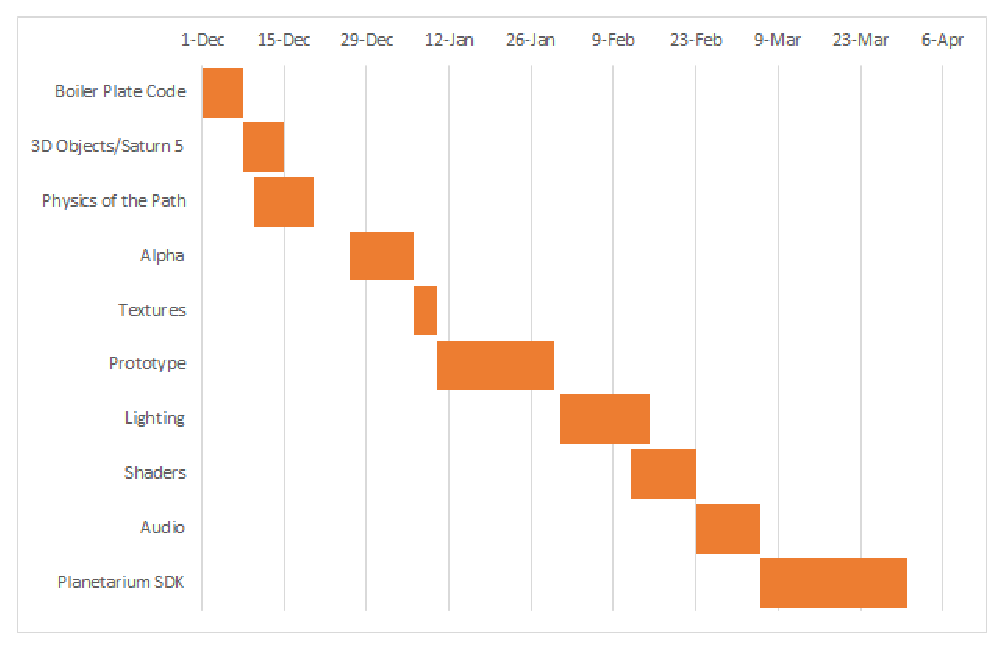
\includegraphics[width=\linewidth]{Gantt.eps}
    \caption{Original gantt chart of proposed timeline}
    \label{fig:Gantt Chart}
\end{figure}

\end{document}